\begin{enumerate}[label=\thesection.\arabic*.,ref=\thesection.\theenumi]
\numberwithin{equation}{enumi}

\begin{abstract}
This document contains the solution complex numbers problem.
\end{abstract}
Download all python codes from 
%
\begin{lstlisting}
https://github.com/sahilsin/MatrixTheory/Assignment1/codes
\end{lstlisting}

\section{Problem}

Convert the following in Polar form:

\begin{align}
        a)  \cfrac{\myvec{1 \\ 7}}{\myvec{2 \\ -1}^{2}}
\end{align}

\begin{align}
        b)  \cfrac{\myvec{1 \\ 3}}{\myvec{1 \\ -2}}
\end{align}


\section{Solution}
The \textbf{Approach} is :
\begin{flushleft}
    For finding the polar form we will first simplify the expressions given in problem and after that the polar form of $\myvec{x \\ y}$ will be of two parts. Magnitude and angle. Magnitude will be $\sqrt{x^2 + y^2}$ and angle will be $\arctan\cfrac{y}{x}$.
\end{flushleft}

\begin{enumerate}
    \item We first convert given problem into simpler form:

\begin{align}
    \cfrac{\myvec{1 \\ 7}}{\myvec{2 \\ -1}^{2}}\\
\end{align} 

We know that :
\begin{align}
    \myvec{a1 \\ a2} = \myvec{a1 & -a2\\a2 & a1}\myvec{1 \\ 0}
\end{align}
The denominator can be simplified as :
\begin{align}
    \myvec{2 \\ -1}^2 = \myvec{2 & 1\\-1 & 2}\myvec{2 & 1\\-1 & 2}\myvec{1 \\ 0}
\\ \\
    \implies \myvec{2 \\ -1}^2 = \myvec{3 & 4\\-4 & 3}\myvec{1 \\ 0}
\\ \\
    \implies \myvec{2 \\ -1}^2 = \myvec{3 \\-4}
\end{align}

Now our Expression becomes :
\begin{align}
    \myvec{1 \\ 7}\myvec{3\\-4}^{-1}
\end{align}

Inverse can be calculated as:
\begin{align}
    \myvec{x \\ y}^{-1}=\cfrac{1}{x^2+y^2}\myvec{x\\-y}
\end{align}

Our problem can now be written as :
\begin{align}
    \cfrac{1}{25}\myvec{1 \\ 7}\myvec{3\\4}
\\
    \implies \cfrac{1}{25}\myvec{1 \\ 7}\myvec{3\\4}
\end{align}

it can be further expanded as :
\begin{align}
    \implies \cfrac{1}{25}\myvec{1 & -7\\7 & 1}\myvec{3 & -4\\4 & 3}\myvec{1 \\ 0}
\\
    \implies \cfrac{1}{25}\myvec{-25 & -25\\25 & -25}\myvec{1 \\ 0}
\\
    \implies \cfrac{1}{25}\myvec{-25 \\ 25}
\end{align}

After further simplifying :
\begin{align}
    \implies \cfrac{25 \times \sqrt{2}}{25}\myvec{-25 \\ 25}
\end{align}

polar form is :
\begin{align}
    \implies \sqrt{2}\arctan\cfrac{25}{-25}
\\
    \implies \sqrt{2} \angle -45 \degree
\end{align}



\item We first convert given problem into simpler form:

\begin{align}
    \cfrac{\myvec{1 \\ 3}}{\myvec{1 \\ -2}}
\end{align} 

We know that :
\begin{align}
    \myvec{a1 \\ a2} = \myvec{a1 & -a2\\a2 & a1}\myvec{1 \\ 0}
\end{align}
The denominator can be simplified as :
\begin{align}
    \myvec{1 \\ -2} = \myvec{1 & 2\\-2 & 1}\myvec{1 \\ 0}
\end{align}

Now our Expression becomes :
\begin{align}
    \myvec{1 \\ 7}\myvec{1\\-2}^{-1}
\end{align}

Inverse can be calculated as:
\begin{align}
    \myvec{x \\ y}^{-1}=\cfrac{1}{x^2+y^2}\myvec{x\\-y}
\end{align}

Our problem can now be written as :
\begin{align}
    \cfrac{1}{5}\myvec{1 \\ 3}\myvec{1\\2}\myvec{1\\0}
\end{align}

it can be further expanded as :
\begin{align}
    \implies \cfrac{1}{5}\myvec{1 & -3\\3 & 1}\myvec{1 & -2\\2 & 1}\myvec{1 \\ 0}
\\
    \implies \cfrac{1}{5}\myvec{-5 & -5\\5 & -5}\myvec{1 \\ 0}
\\
    \implies \cfrac{1}{5}\myvec{-5 \\ 5}
\end{align}

After further simplifying :
\begin{align}
    \implies \cfrac{5 \times \sqrt{2}}{5}\myvec{-5 \\ 5}
\end{align}

polar form is :
\begin{align}
    \implies \sqrt{2}\arctan\cfrac{5}{-5}
\\
    \implies \sqrt{2} \angle -45 \degree
\end{align}

For both the part as our polar forms comes to be same , it will look like a line having magnitude as $\sqrt{2}$ and angle as $-45\degree$
,so it will look like a line $\myvec{1 \\ 1}=0$ as shown :

\renewcommand{\thefigure}{\theenumi.\arabic{figure}}
\begin{figure}[!ht]
    \centering
    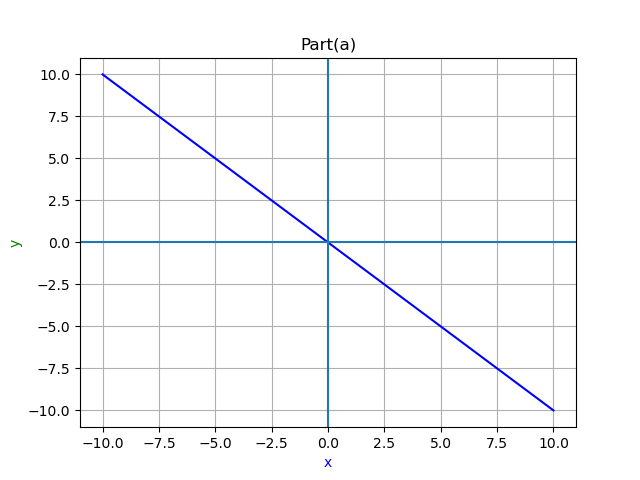
\includegraphics[width=\columnwidth]{./figures/MT_A1_a}
\caption{part(a)}
\label{fig: part(a)}
\end{figure}

\end{enumerate}

\end{enumerate}


